
\documentclass[11pt, a4paper, twocolumn]{article}

% --- UNIVERSAL PREAMBLE BLOCK ---
\usepackage[a4paper, top=2.5cm, bottom=2.5cm, left=2cm, right=2cm]{geometry}
\usepackage{fontspec}

\usepackage[english, bidi=basic, provide=*]{babel}

\babelprovide[import, onchar=ids fonts]{english}

% Set default/Latin font to Sans Serif in the main (rm) slot
\babelfont{rm}{Noto Sans}

% --- REQUIRED PACKAGES ---
\usepackage{amsmath}
\usepackage{booktabs}
\usepackage{graphicx}
\usepackage{hyperref} % Must be the last package loaded

% --- TEMPLATE COMPATIBILITY MACROS ---
% These macros allow the iLCSS custom template tags to compile natively 
% in a standard LaTeX environment without requiring the external ilcss.cls file.
\usepackage{authblk}
\newcommand{\templatetype}[1]{}
\newcommand{\leadauthor}[1]{}

\newcommand{\storedsig}{}
\newcommand{\significancestatement}[1]{\renewcommand{\storedsig}{\vspace{1em}\noindent\textbf{Significance Statement: } #1 \par\vspace{1em}}}

\newcommand{\authorcontributions}[1]{}
\newcommand{\authordeclaration}[1]{}
\newcommand{\equalauthors}[1]{}

\newcommand{\storedcorr}{}
\newcommand{\correspondingauthor}[1]{\renewcommand{\storedcorr}{\vspace{1em}\noindent\textit{#1}\par}}

\newcommand{\storedkeys}{}
\newcommand{\keywords}[1]{\renewcommand{\storedkeys}{\noindent\textbf{Keywords: } #1 \par\vspace{1em}}}

\newcommand{\storeddates}{}
\newcommand{\dates}[1]{\renewcommand{\storeddates}{\vspace{1em}\noindent\textit{#1}\par}}

\newcommand{\doi}[1]{}
\newcommand{\dropcap}[1]{\noindent\textbf{\Large #1}}
\newcommand{\acknow}[1]{\section*{Acknowledgments} #1}
\newcommand{\showacknow}{}

\let\oldmaketitle\maketitle
\renewcommand{\maketitle}{%
  \oldmaketitle
  \storedsig
  \storedcorr
  \storedkeys
  \storeddates
}

% --- DOCUMENT METADATA ---
\templatetype{ilcssworkingpaper}

\title{Projecting the Macroeconomic Impact of Artificial Intelligence on Municipal Economies: A 2050 Scenario Analysis for Kota Denpasar}

% Use letters for affiliations, numbers to show equal authorship (if applicable) and to indicate the corresponding author
\author[1,2*]{Ricardo Ochoa}
\author[1]{Socorro Román}

\affil[1]{CAPSUS}

\leadauthor{ricardo.ochoa@capsus.mx}

\significancestatement{As artificial intelligence shifts from theoretical modeling to active structural integration, its macroeconomic impacts on urban centers in developing economies remain largely uncharted. This study projects the trajectory of Denpasar, Indonesia, revealing a potential 60 trillion Rupiah 'AI Dividend' by 2050. However, it also uncovers a critical threat of severe wage polarization between formal, AI-augmented workers and the informal labor sector. These findings provide essential localized data for policymakers, emphasizing that aggressive, universal digital upskilling is required to prevent widespread economic inequality as municipal economies transition into the AI era.}

\authorcontributions{R.O. designed the research architecture and developed the macroeconomic projection model. S.R. performed data collection, baseline triangulation, and spatial analysis. Both authors contributed to writing and reviewing the final manuscript.}
\authordeclaration{The authors declare no conflict of interest.}
\correspondingauthor{\textsuperscript{2} E-mail: ricardo.ochoa@capsus.mx}

\keywords{Artificial Intelligence $|$ Urban Economics $|$ Shift-Share Analysis $|$ Technological Diffusion $|$ Kota Denpasar}

\dates{This manuscript was compiled on \today}

\doi{\url{http://ilcss.umd.edu/}}

\begin{document}

\maketitle

\begin{abstract}
The rapid evolution of artificial intelligence (AI) and automation has shifted from theoretical modeling to structural enterprise integration, generating unprecedented macroeconomic consequences. While global and national forecasts abound, urban municipalities serve as the primary nodes for technological diffusion and labor market transitions. This working paper introduces a localized, micro-to-macro modeling architecture to project the economic impact of AI on Kota Denpasar, Indonesia, through 2050. Utilizing a task-based labor exposure index triangulated with recent municipal data, we establish a baseline for Denpasar's highly formalized, service-oriented economy. We apply logistic diffusion models (S-curves) adjusted for local frictions and accelerators, mapping these onto projected Total Factor Productivity (TFP) shocks. Our results indicate a bifurcated future: under a High Transformation scenario, AI integration yields a "productivity dividend" pushing municipal GRDP to 195 Trillion IDR by 2050, but concurrently triggers severe wage polarization between formal "augmented" workers and the informal sector. The paper concludes with policy implications for navigating this technological transition.
\end{abstract}
%------------------------

\dropcap{T}he integration of generative artificial intelligence (AI) and advanced automation into the global economy represents a paradigm shift in the mechanisms of value creation. Unlike previous technological revolutions that primarily substituted routine physical labor, the current wave of AI demonstrates a profound capacity to augment or replace cognitive, non-routine, and knowledge-intensive tasks. In the East Asia and Pacific (EAP) region, digital transformation is enhancing the tradability of services and redefining production processes, as highlighted by recent assessments of future job landscapes \cite{worldbank2025}.

However, estimating the long-term macroeconomic consequences of these technologies requires moving beyond generalized national forecasts to highly granular, municipal-level projections. Urban centers are the arenas where capital accumulation, digital infrastructure, and labor market transitions intersect. An urban municipality in Southeast Asia will not experience AI adoption uniformly; the trajectory is dictated by localized industrial composition, labor informality, and specific digital infrastructure readiness.

This paper applies a localized projection framework to Kota Denpasar, the capital of Bali Province, Indonesia. With a 2024 Gross Regional Domestic Product (GRDP) of 38.00 Trillion IDR (at constant prices) heavily dominated by the Accommodation, Food Service, and Education sectors \cite{bps2025_pdrb}, Denpasar presents a unique case study. Unlike the national average, Denpasar exhibits a remarkably high formal employment rate (61.8\%) and near-universal 4G/5G connectivity. This research answers a critical question: \textit{How will the structural integration of AI alter Denpasar's economic output and wage distribution by 2050?}

\section*{Theoretical Background}
The theoretical foundation of this projection relies on three interconnected economic frameworks:

\subsection*{The Task-Based Model of Automation}
Traditional models of technological change assume that technology universally augments labor. This paper adopts the task-based framework pioneered by Autor, Levy, and Murnane \cite{autor2003} and expanded by Acemoglu and Restrepo \cite{acemoglu2018}. In this model, production requires the completion of a continuum of tasks. AI does not replace "jobs" entirely; rather, it substitutes human labor in specific cognitive and routine tasks while complementing human labor in others (augmentation). The exposure of a municipality's workforce is therefore a function of its task composition.
  
\subsection*{Technological Diffusion and S-Curves}
The adoption of general-purpose technologies (GPTs) follows a logistic growth curve, or S-curve, characterized by a slow incubation period, rapid exponential acceleration (the tipping point), and eventual saturation \cite{griliches1957}. For AI, the steepness and timing of this curve are mediated by local "frictions" (e.g., labor informality, lack of digital infrastructure) and "accelerators" (e.g., public sector digitization pilots, blanket 5G coverage).
  
\subsection*{Skill-Biased Technological Change and Wage Polarization}
As established in labor economics, technologies that complement highly skilled workers increase their marginal productivity and wages, while displacing middle-skill routine workers. In the context of a developing economy like Indonesia, this dynamic manifests as a polarization between the formal sector (which captures the AI augmentation dividend) and the informal sector (which remains shielded from direct automation but suffers from wage stagnation).
  
\section*{Methodology and Assumptions}
To model Denpasar's trajectory to 2050, we employ a three-phase analytical sequence relying on data triangulation from Statistics Indonesia (BPS) \cite{bps2025_denpasar}.

\subsection*{Data Triangulation and Baseline}
Because direct corporate tech integration metrics are not fully mature, we triangulate baseline digital readiness using proxy indicators:
\begin{itemize}
    \item \textbf{Sectoral Composition:} Extracted from the 2024 GRDP by Industry report, showing Services as the dominant economic anchor.
    \item \textbf{Labor Dynamics:} Sourced from the August 2025 National Labor Force Survey (Sakernas), identifying a workforce of 411,042 individuals (61.8\% formal, 38.2\% informal) \cite{bps2026_sakernas}.
    \item \textbf{Digital Footprint:} E-Commerce Statistics (2024) indicating 51.37\% e-commerce adoption among local enterprises \cite{bps2025_ecommerce} and 100\% broadband coverage across Denpasar's wards.
\end{itemize}
  
\subsection*{Phase 1: Occupational Exposure Assessment}
We utilize a Shift-Share Analysis combined with an AI Task-Exposure Index. As illustrated in Figure \ref{fig:exposure}, the workers in Denpasar are categorized into three exposure tiers based on their primary sectors.

\begin{figure}[tbhp]
  \centering
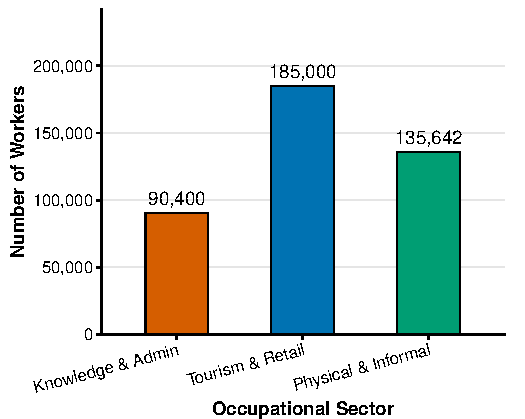
\includegraphics[width=\linewidth]{img/Denpasar_Phase1_Exposure_Academic.pdf}  \caption{Denpasar labor force AI exposure by occupational sector (2024 Baseline).}
  \label{fig:exposure}
\end{figure}

The tiers include High Exposure for Knowledge \& Admin sectors ($\sim$90,400 workers), Medium Exposure for Tourism \& Retail ($\sim$185,000 workers), and Low Exposure for Physical \& Informal labor ($\sim$135,600 workers).
  
\subsection*{Phase 2: Temporal Diffusion Modeling}
We model the speed of task transition using logistic growth functions parameterized for local conditions. The adoption rate $A(t)$ for sector $i$ in year $t$ is defined as:
\begin{equation}
  A_i(t) = \frac{L_i}{1 + e^{-k_i (t - t_{0,i} - \alpha)}}
  \label{eqn:diffusion}
\end{equation}
Where $L$ is the maximum adoption saturation limit, $k$ is the diffusion speed, $t_0$ is the base tipping point year, and $\alpha$ represents local acceleration factors. For Denpasar, $\alpha$ is adjusted to reflect the late 2025 deployment of blanket 5G and the 2026 provincial single digital identity pilot. Figure \ref{fig:diffusion} displays the modeled adoption rates.

\begin{figure}[tbhp]
  \centering
  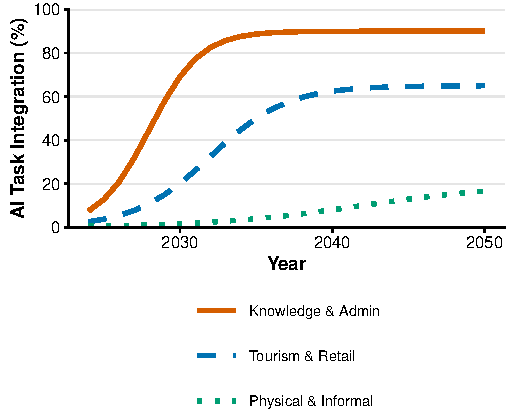
\includegraphics[width=\linewidth]{img/Denpasar_Phase2_SCurves_Academic.pdf} 
  \caption{AI temporal diffusion S-Curves by occupational sector, accelerated by local digital infrastructure readiness.}
  \label{fig:diffusion}
\end{figure}
  
\subsection*{Phase 3: Macroeconomic Projections}
We translate localized task-exposure and diffusion timelines into macroeconomic Total Factor Productivity (TFP) shocks. These shocks are fed into a dynamic projection model to calculate the potential bounds of municipal GRDP and the divergence in the wage inequality index.
  
\section*{Results and Discussion}
  
\subsection*{The Productivity Dividend}
The modeling reveals a massive divergence in Denpasar's potential economic size by 2050 based on the rate of AI adoption. As shown in Figure \ref{fig:grdp}, the trajectory varies drastically depending on local integration efforts.

\begin{figure}[tbhp]
  \centering
    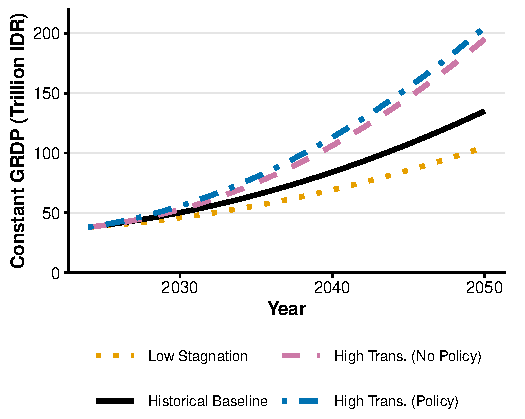
\includegraphics[width=\linewidth]{img/Denpasar_Phase3_GRDP_Academic.pdf} 
  \caption{Projected Municipal GRDP to 2050 mapped across four automation and policy scenarios.}
  \label{fig:grdp}
\end{figure}

In the \textit{High Transformation} scenarios, the aggressive integration of AI adds an estimated 1.2\% to 1.8\% to annual TFP growth starting in the early 2030s. This yields an "AI Dividend" of approximately 60 Trillion IDR over the historical baseline by 2050. Conversely, failure to adopt these technologies (\textit{Low Adoption}) leads to severe competitive degradation.
  
\subsection*{Wage Polarization and the Inequality Threat}
While AI significantly expands aggregate output, the distribution of this wealth is structurally biased. Denpasar's informal sector lacks the capital to integrate AI. 

As detailed in Figure \ref{fig:ineq}, without structural intervention, the wage inequality index will spike severely between 2035 and 2045. The "augmented" formal workers in tourism and administration will see exponential productivity gains, while informal workers will experience real-wage stagnation.

\begin{figure}[tbhp]
  \centering
        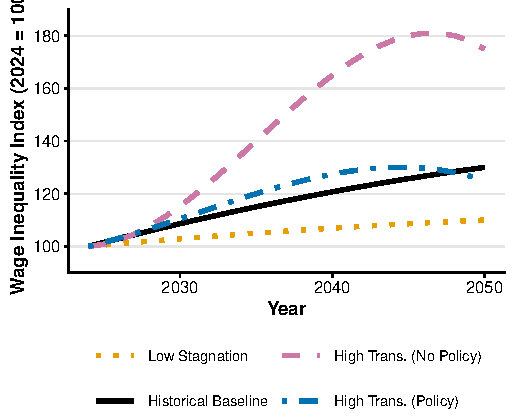
\includegraphics[width=\linewidth]{img/Denpasar_Phase3_Inequality_Academic.pdf} 
  \caption{Wage Inequality Index projections illustrating the polarization risk between formal and informal labor tiers.}
  \label{fig:ineq}
\end{figure}

\subsection*{Spatial and Urban Dynamics}
The macroeconomic shifts will alter Denpasar's spatial layout. The automation of routine administrative tasks will likely contract demand for traditional centralized commercial real estate. Simultaneously, the demand for decentralized, high-connectivity co-working nodes for hybrid "human-AI" teams will drive development outward.
  
\section*{Conclusion and Policy Implications}
The trajectory of Kota Denpasar to 2050 highlights both the immense potential and structural risks of the AI revolution. Because of its unique demographic and infrastructure profile, Denpasar is positioned to capture a disproportionately large AI productivity dividend.
  
However, capturing this 195 Trillion IDR economy requires preemptive policy action. To mitigate the severe wage polarization identified in the projection, municipal authorities must implement aggressive, universal digital upskilling programs targeting both the formal and informal sectors. Successfully navigating this transition will be critical to fulfilling the ambitions of the "Golden Indonesia 2045" roadmaps.

\acknow{We thank the members of the CAPSUS data analytics team for their valuable feedback and support during the data compilation and parameterization phases of this project.}

\showacknow{}

% Bibliography
% Included inline to ensure single-file compilation without requiring external .bib files
\begin{thebibliography}{99}
  
\bibitem{acemoglu2018}
Acemoglu, D., \& Restrepo, P. (2018). The Race between Man and Machine: Implications of Technology for Growth, Factor Shares, and Employment. \textit{American Economic Review}, 108(6), 1488-1542.
  
\bibitem{autor2003}
Autor, D. H., Levy, F., \& Murnane, R. J. (2003). The Skill Content of Recent Technological Change: An Empirical Exploration. \textit{The Quarterly Journal of Economics}, 118(4), 1279-1333.
  
\bibitem{bps2025_denpasar}
Badan Pusat Statistik Kota Denpasar. (2025). \textit{Kota Denpasar Dalam Angka 2025 [Denpasar Municipality in Figures 2025]}. BPS-Statistics Denpasar Municipality.
  
\bibitem{bps2025_pdrb}
Badan Pusat Statistik Kota Denpasar. (2025). \textit{Produk Domestik Regional Bruto Kota Denpasar Menurut Lapangan Usaha 2020-2024}. BPS-Statistics Denpasar Municipality.
  
\bibitem{bps2026_sakernas}
Badan Pusat Statistik. (2026). \textit{Booklet Sakernas Agustus 2025}. BPS-Statistics Indonesia.
  
\bibitem{bps2025_ecommerce}
Badan Pusat Statistik. (2025). \textit{Statistik E-Commerce 2024}. BPS-Statistics Indonesia.
  
\bibitem{griliches1957}
Griliches, Z. (1957). Hybrid Corn: An Exploration in the Economics of Technological Change. \textit{Econometrica}, 25(4), 501-522.
  
\bibitem{worldbank2025}
World Bank Group. (2025). \textit{Future Jobs: Robots, Artificial Intelligence, and Digital Platforms in East Asia and Pacific}. East Asia and Pacific Development Studies. Washington, DC: World Bank.
  
\bibitem{worldbank2016}
World Bank Group. (2016). \textit{Live Long and Prosper: Aging in East Asia and Pacific}. World Bank East Asia and Pacific Regional Report. Washington, DC: World Bank.
  
\end{thebibliography}

\end{document}